\section{eo\-Es\-Mutate$<$ EOT $>$ Class Template Reference}
\label{classeo_es_mutate}\index{eoEsMutate@{eoEsMutate}}
ES-style mutation in the large.  


{\tt \#include $<$eo\-Es\-Mutate.h$>$}

Inheritance diagram for eo\-Es\-Mutate$<$ EOT $>$::\begin{figure}[H]
\begin{center}
\leavevmode
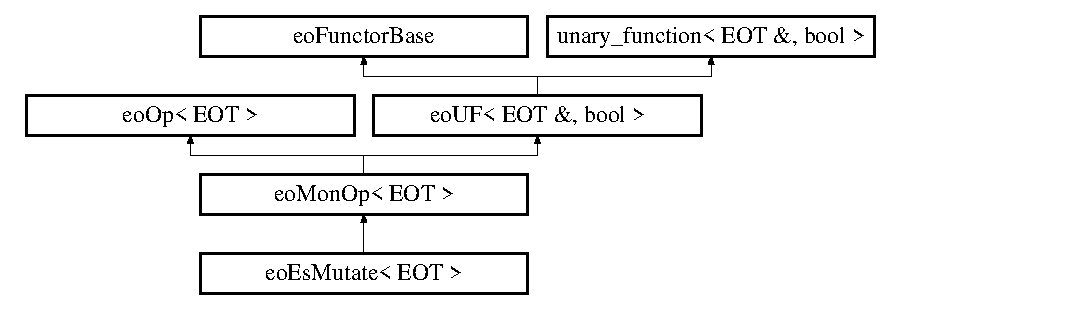
\includegraphics[height=3.71476cm]{classeo_es_mutate}
\end{center}
\end{figure}
\subsection*{Public Types}
\begin{CompactItemize}
\item 
typedef EOT::Fitness {\bf Fit\-T}\label{classeo_es_mutate_w0}

\begin{CompactList}\small\item\em Fitness-type. \item\end{CompactList}\end{CompactItemize}
\subsection*{Public Member Functions}
\begin{CompactItemize}
\item 
{\bf eo\-Es\-Mutate} ({\bf eo\-Es\-Mutation\-Init} \&\_\-init, {\bf eo\-Real\-Vector\-Bounds} \&\_\-bounds)
\begin{CompactList}\small\item\em Initialization. \item\end{CompactList}\item 
virtual {\bf $\sim$eo\-Es\-Mutate} ()\label{classeo_es_mutate_a1}

\begin{CompactList}\small\item\em Virtual Destructor. \item\end{CompactList}\item 
virtual std::string {\bf class\-Name} () const 
\begin{CompactList}\small\item\em Classname. \item\end{CompactList}\item 
virtual bool {\bf operator()} ({\bf eo\-Es\-Simple}$<$ {\bf Fit\-T} $>$ \&\_\-eo)
\begin{CompactList}\small\item\em Mutate {\bf eo\-Es\-Simple}{\rm (p.\,\pageref{classeo_es_simple})}. \item\end{CompactList}\item 
virtual bool {\bf operator()} ({\bf eo\-Es\-Stdev}$<$ {\bf Fit\-T} $>$ \&\_\-eo)
\begin{CompactList}\small\item\em Standard mutation in ES. \item\end{CompactList}\item 
virtual bool {\bf operator()} ({\bf eo\-Es\-Full}$<$ {\bf Fit\-T} $>$ \&\_\-eo)
\begin{CompactList}\small\item\em Correlated mutations in ES. \item\end{CompactList}\end{CompactItemize}
\subsection*{Private Member Functions}
\begin{CompactItemize}
\item 
void {\bf init} ({\bf eo\-Es\-Simple}$<$ {\bf Fit\-T} $>$, {\bf eo\-Es\-Mutation\-Init} \&\_\-init)\label{classeo_es_mutate_d0}

\begin{CompactList}\small\item\em Initialization of simple ES. \item\end{CompactList}\item 
void {\bf init} ({\bf eo\-Es\-Stdev}$<$ {\bf Fit\-T} $>$, {\bf eo\-Es\-Mutation\-Init} \&\_\-init)
\begin{CompactList}\small\item\em Initialization of standard ES. \item\end{CompactList}\item 
void {\bf init} ({\bf eo\-Es\-Full}$<$ {\bf Fit\-T} $>$, {\bf eo\-Es\-Mutation\-Init} \&\_\-init)
\begin{CompactList}\small\item\em Initialization of full ES. \item\end{CompactList}\end{CompactItemize}
\subsection*{Private Attributes}
\begin{CompactItemize}
\item 
double {\bf Tau\-Lcl}\label{classeo_es_mutate_r0}

\begin{CompactList}\small\item\em Local factor for mutation of std deviations. \item\end{CompactList}\item 
double {\bf Tau\-Glb}\label{classeo_es_mutate_r1}

\begin{CompactList}\small\item\em Global factor for mutation of std deviations. \item\end{CompactList}\item 
double {\bf Tau\-Beta}\label{classeo_es_mutate_r2}

\begin{CompactList}\small\item\em Factor for mutation of correlation parameters. \item\end{CompactList}\item 
{\bf eo\-Real\-Vector\-Bounds} \& {\bf bounds}\label{classeo_es_mutate_r3}

\begin{CompactList}\small\item\em Bounds of parameters. \item\end{CompactList}\end{CompactItemize}
\subsection*{Static Private Attributes}
\begin{CompactItemize}
\item 
const double {\bf stdev\_\-eps} = 1.0e-40
\begin{CompactList}\small\item\em Minimum stdev. \item\end{CompactList}\end{CompactItemize}


\subsection{Detailed Description}
\subsubsection*{template$<$class EOT$>$ class eo\-Es\-Mutate$<$ EOT $>$}

ES-style mutation in the large. 

Obviously, valid only for eo\-ES$\ast$. It is currently valid for three types of ES chromosomes:\begin{itemize}
\item {\bf eo\-Es\-Simple}{\rm (p.\,\pageref{classeo_es_simple})}: Exactly one stdandard-deviation\item {\bf eo\-Es\-Stdev}{\rm (p.\,\pageref{classeo_es_stdev})}: As many standard deviations as object variables\item {\bf eo\-Es\-Full}{\rm (p.\,\pageref{classeo_es_full})}: The whole guacemole: correlations, stdevs and object variables\end{itemize}


Each of these three variant has it's own operator() in eo\-Es\-Mutate and intialization is also split into three cases (that share some commonalities) 



Definition at line 60 of file eo\-Es\-Mutate.h.

\subsection{Constructor \& Destructor Documentation}
\index{eoEsMutate@{eo\-Es\-Mutate}!eoEsMutate@{eoEsMutate}}
\index{eoEsMutate@{eoEsMutate}!eoEsMutate@{eo\-Es\-Mutate}}
\subsubsection{\setlength{\rightskip}{0pt plus 5cm}template$<$class EOT$>$ {\bf eo\-Es\-Mutate}$<$ {\bf EOT} $>$::{\bf eo\-Es\-Mutate} ({\bf eo\-Es\-Mutation\-Init} \& {\em \_\-init}, {\bf eo\-Real\-Vector\-Bounds} \& {\em \_\-bounds})\hspace{0.3cm}{\tt  [inline]}}\label{classeo_es_mutate_a0}


Initialization. 

\begin{Desc}
\item[Parameters:]
\begin{description}
\item[{\em \_\-init}]Proxy class for initializating the three parameters eo\-Es\-Mutate needs \item[{\em \_\-bounds}]Bounds for the objective variables \end{description}
\end{Desc}


Definition at line 74 of file eo\-Es\-Mutate.h.

References eo\-Es\-Mutate$<$ EOT $>$::bounds, and eo\-Es\-Mutate$<$ EOT $>$::init().

\subsection{Member Function Documentation}
\index{eoEsMutate@{eo\-Es\-Mutate}!className@{className}}
\index{className@{className}!eoEsMutate@{eo\-Es\-Mutate}}
\subsubsection{\setlength{\rightskip}{0pt plus 5cm}template$<$class EOT$>$ virtual std::string {\bf eo\-Es\-Mutate}$<$ {\bf EOT} $>$::class\-Name (void) const\hspace{0.3cm}{\tt  [inline, virtual]}}\label{classeo_es_mutate_a2}


Classname. 

Inherited from {\bf eo\-Object}{\rm (p.\,\pageref{classeo_object})} \begin{Desc}
\item[See also:]{\bf eo\-Object}{\rm (p.\,\pageref{classeo_object})}\end{Desc}
\begin{Desc}
\item[Returns:]Name of class. \end{Desc}


Reimplemented from {\bf eo\-Mon\-Op$<$ EOT $>$} {\rm (p.\,\pageref{classeo_mon_op})}.

Definition at line 90 of file eo\-Es\-Mutate.h.\index{eoEsMutate@{eo\-Es\-Mutate}!operator()@{operator()}}
\index{operator()@{operator()}!eoEsMutate@{eo\-Es\-Mutate}}
\subsubsection{\setlength{\rightskip}{0pt plus 5cm}template$<$class EOT$>$ virtual bool {\bf eo\-Es\-Mutate}$<$ {\bf EOT} $>$::operator() ({\bf eo\-Es\-Simple}$<$ {\bf Fit\-T} $>$ \& {\em \_\-eo})\hspace{0.3cm}{\tt  [inline, virtual]}}\label{classeo_es_mutate_a3}


Mutate {\bf eo\-Es\-Simple}{\rm (p.\,\pageref{classeo_es_simple})}. 

\begin{Desc}
\item[Parameters:]
\begin{description}
\item[{\em \_\-eo}]Individual to mutate. \end{description}
\end{Desc}


Definition at line 97 of file eo\-Es\-Mutate.h.

References eo\-Es\-Mutate$<$ EOT $>$::bounds, eo\-Real\-Base\-Vector\-Bounds::folds\-In\-Bounds(), eo\-Rng::normal(), eo\-Es\-Simple$<$ Fit $>$::stdev, and eo\-Es\-Mutate$<$ EOT $>$::Tau\-Lcl.\index{eoEsMutate@{eo\-Es\-Mutate}!operator()@{operator()}}
\index{operator()@{operator()}!eoEsMutate@{eo\-Es\-Mutate}}
\subsubsection{\setlength{\rightskip}{0pt plus 5cm}template$<$class EOT$>$ virtual bool {\bf eo\-Es\-Mutate}$<$ {\bf EOT} $>$::operator() ({\bf eo\-Es\-Stdev}$<$ {\bf Fit\-T} $>$ \& {\em \_\-eo})\hspace{0.3cm}{\tt  [inline, virtual]}}\label{classeo_es_mutate_a4}


Standard mutation in ES. 

This is an overloaded member function, provided for convenience. It differs from the above function only in what argument(s) it accepts.

Standard mutation of object variables and standard deviations in ESs.

If there are fewer different standard deviations available than the dimension of the objective function requires, the last standard deviation is responsible for ALL remaining object variables.

\begin{Desc}
\item[Parameters:]
\begin{description}
\item[{\em \_\-eo}]Individual to mutate.\end{description}
\end{Desc}
\begin{Desc}
\item[See also:]Schwefel 1977: Numerische Optimierung von Computer-Modellen mittels der Evolutionsstrategie, pp. 165 ff. \end{Desc}


Definition at line 128 of file eo\-Es\-Mutate.h.

References eo\-Es\-Mutate$<$ EOT $>$::bounds, eo\-Real\-Base\-Vector\-Bounds::folds\-In\-Bounds(), eo\-Rng::normal(), eo\-Es\-Stdev$<$ Fit $>$::stdevs, eo\-Es\-Mutate$<$ EOT $>$::Tau\-Glb, and eo\-Es\-Mutate$<$ EOT $>$::Tau\-Lcl.\index{eoEsMutate@{eo\-Es\-Mutate}!operator()@{operator()}}
\index{operator()@{operator()}!eoEsMutate@{eo\-Es\-Mutate}}
\subsubsection{\setlength{\rightskip}{0pt plus 5cm}template$<$class EOT$>$ virtual bool {\bf eo\-Es\-Mutate}$<$ {\bf EOT} $>$::operator() ({\bf eo\-Es\-Full}$<$ {\bf Fit\-T} $>$ \& {\em \_\-eo})\hspace{0.3cm}{\tt  [inline, virtual]}}\label{classeo_es_mutate_a5}


Correlated mutations in ES. 

This is an overloaded member function, provided for convenience. It differs from the above function only in what argument(s) it accepts.

Mutation of object variables, standard deviations, and their correlations in ESs.

\begin{Desc}
\item[Parameters:]
\begin{description}
\item[{\em \_\-eo}]Individual to mutate.\end{description}
\end{Desc}
\begin{Desc}
\item[See also:]\begin{itemize}
\item H.-P. Schwefel: Internal Report of KFA Juelich, KFA-STE-IB-3/80, p. 43, 1980.\item G. Rudolph: Globale Optimierung mit parallelen Evolutionsstrategien, Diploma Thesis, University of Dortmund, 1990. \end{itemize}
\end{Desc}


Definition at line 159 of file eo\-Es\-Mutate.h.

References eo\-Es\-Mutate$<$ EOT $>$::bounds, eo\-Es\-Full$<$ Fit $>$::correlations, eo\-Real\-Base\-Vector\-Bounds::folds\-In\-Bounds(), eo\-Rng::normal(), eo\-Es\-Full$<$ Fit $>$::stdevs, eo\-Es\-Mutate$<$ EOT $>$::Tau\-Beta, eo\-Es\-Mutate$<$ EOT $>$::Tau\-Glb, and eo\-Es\-Mutate$<$ EOT $>$::Tau\-Lcl.\index{eoEsMutate@{eo\-Es\-Mutate}!init@{init}}
\index{init@{init}!eoEsMutate@{eo\-Es\-Mutate}}
\subsubsection{\setlength{\rightskip}{0pt plus 5cm}template$<$class EOT$>$ void {\bf eo\-Es\-Mutate}$<$ {\bf EOT} $>$::init ({\bf eo\-Es\-Stdev}$<$ {\bf Fit\-T} $>$, {\bf eo\-Es\-Mutation\-Init} \& {\em \_\-init})\hspace{0.3cm}{\tt  [inline, private]}}\label{classeo_es_mutate_d1}


Initialization of standard ES. 

This is an overloaded member function, provided for convenience. It differs from the above function only in what argument(s) it accepts. 

Definition at line 228 of file eo\-Es\-Mutate.h.

References eo\-Es\-Mutate$<$ EOT $>$::bounds, eo\-Es\-Mutation\-Init::Tau\-Glb(), eo\-Es\-Mutate$<$ EOT $>$::Tau\-Glb, eo\-Es\-Mutation\-Init::Tau\-Lcl(), and eo\-Es\-Mutate$<$ EOT $>$::Tau\-Lcl.\index{eoEsMutate@{eo\-Es\-Mutate}!init@{init}}
\index{init@{init}!eoEsMutate@{eo\-Es\-Mutate}}
\subsubsection{\setlength{\rightskip}{0pt plus 5cm}template$<$class EOT$>$ void {\bf eo\-Es\-Mutate}$<$ {\bf EOT} $>$::init ({\bf eo\-Es\-Full}$<$ {\bf Fit\-T} $>$, {\bf eo\-Es\-Mutation\-Init} \& {\em \_\-init})\hspace{0.3cm}{\tt  [inline, private]}}\label{classeo_es_mutate_d2}


Initialization of full ES. 

This is an overloaded member function, provided for convenience. It differs from the above function only in what argument(s) it accepts. 

Definition at line 244 of file eo\-Es\-Mutate.h.

References eo\-Es\-Mutate$<$ EOT $>$::init(), eo\-Es\-Mutation\-Init::Tau\-Beta(), eo\-Es\-Mutate$<$ EOT $>$::Tau\-Beta, eo\-Es\-Mutate$<$ EOT $>$::Tau\-Glb, and eo\-Es\-Mutate$<$ EOT $>$::Tau\-Lcl.

\subsection{Member Data Documentation}
\index{eoEsMutate@{eo\-Es\-Mutate}!stdev_eps@{stdev\_\-eps}}
\index{stdev_eps@{stdev\_\-eps}!eoEsMutate@{eo\-Es\-Mutate}}
\subsubsection{\setlength{\rightskip}{0pt plus 5cm}template$<$class EOT$>$ const double {\bf eo\-Es\-Mutate}$<$ {\bf EOT} $>$::{\bf stdev\_\-eps} = 1.0e-40\hspace{0.3cm}{\tt  [static, private]}}\label{classeo_es_mutate_v0}


Minimum stdev. 

If you let the step-size go to 0, self-adaptation stops, therefore we give a lower bound. The actual value used is somewhat arbitrary and the is no theoretical reasoning known for it (Sep 2005).

The code that we have in {\bf EO}{\rm (p.\,\pageref{class_e_o})} is a port from a C code that Thomas B\"{a}ck kindly donated to the community some years ago. It has been modified by Marc Schoenauer for inclusion in Evol\-C, than by Maarten Keijzer into {\bf EO}{\rm (p.\,\pageref{class_e_o})}. The exact value was adjusted based on practice.

Removing this doesn't work well, but it was never tried to figure out what the best value would be. 

Definition at line 284 of file eo\-Es\-Mutate.h.

The documentation for this class was generated from the following file:\begin{CompactItemize}
\item 
eo\-Es\-Mutate.h\end{CompactItemize}
